% Erklärung des Designpatterns

\section{Description}

% https://en.wikipedia.org/wiki/Interpreter_pattern

One class for each symbol: 
\begin{itemize}
    \item Terminal
    \item Nonterminal
\end{itemize}


\subsection{Terminal Symbols}
% https://en.wikipedia.org/wiki/Terminal_and_nonterminal_symbols
% https://de.wikipedia.org/wiki/Terminalsymbol

\subsection{Nonterminal Symbols}
% Replacable - nonterminal
% https://en.wikipedia.org/wiki/Terminal_and_nonterminal_symbols
% https://de.wikipedia.org/wiki/Nichtterminalsymbol

\subsection{Abstract Syntax Tree}

]subsubsection{}

For example you have a simple JavaScript function: 
\begin{verbatim}
function foo(x) {
if (x > 10) {
    var a = 2;
    return a * x;
}

return x + 10;
}
\end{verbatim}

\begin{figure}[H]
    \centering
        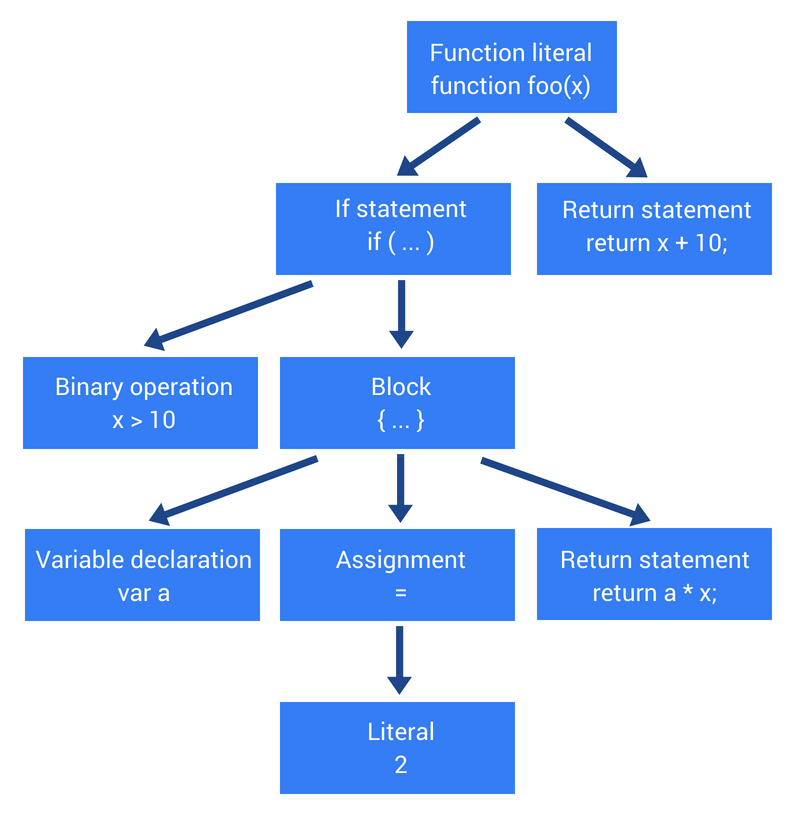
\includegraphics[width=0.8\textwidth]{figures/javascript_ast.png}
\end{figure}

This AST has been simplified for visualization purposes. The actual AST would be much more complex and contain more data. There's a cool project, where you can show the actual AST of a JavaScript program: https://astexplorer.net/

% https://blog.sessionstack.com/how-javascript-works-parsing-abstract-syntax-trees-asts-5-tips-on-how-to-minimize-parse-time-abfcf7e8a0c8

\subsubsection{Usages}

\begin{itemize}
    \item Code Formatters
    \item Extensions for IDEs
\end{itemize}
